%File: GMSWA_AAAI_final.tex
% ============================================================================
% GMSWA --- AAAI anonymous-submission source (FINAL honest version).
%
% BASE KIT NOTICE: produced against the AAAI-2026 Author Kit (aaai2026.sty/.bst,
% AnonymousSubmission/LaTeX). Before submitting to AAAI-27, swap in the official
% aaai2027 kit (sty/bst + \usepackage option + \bibliographystyle) once released
% and re-check the preamble against the AAAI-27 sample, which must be used EXACTLY.
%
% Compile: pdflatex -> bibtex -> pdflatex -> pdflatex
%
% OPEN EXPERIMENTS (text complete; these runs are deferred until GPUs free --
% see TODO_experiments.md). They are flagged with \todo{...} in-line.
% ============================================================================

\documentclass[letterpaper]{article} % DO NOT CHANGE THIS
\usepackage[submission]{aaai2026}  % DO NOT CHANGE THIS  (-> aaai2027 for AAAI-27)
\usepackage{times}  % DO NOT CHANGE THIS
\usepackage{helvet}  % DO NOT CHANGE THIS
\usepackage{courier}  % DO NOT CHANGE THIS
\usepackage[hyphens]{url}  % DO NOT CHANGE THIS
\usepackage{graphicx} % DO NOT CHANGE THIS
\urlstyle{rm} % DO NOT CHANGE THIS
\def\UrlFont{\rm}  % DO NOT CHANGE THIS
\usepackage{natbib}  % DO NOT CHANGE THIS AND DO NOT ADD ANY OPTIONS TO IT
\usepackage{caption} % DO NOT CHANGE THIS AND DO NOT ADD ANY OPTIONS TO IT
\frenchspacing  % DO NOT CHANGE THIS
\setlength{\pdfpagewidth}{8.5in} % DO NOT CHANGE THIS
\setlength{\pdfpageheight}{11in} % DO NOT CHANGE THIS

\usepackage{amsmath}
\usepackage{amssymb}
\usepackage{booktabs}

\DeclareCaptionStyle{ruled}{labelfont=normalfont,labelsep=colon,strut=off} % DO NOT CHANGE THIS

\pdfinfo{
/TemplateVersion (2026.1)
}

\setcounter{secnumdepth}{2}

% TODO marker for deferred (GPU-gated) experiments. Set \todoon to false to hide
% these notes for a clean reading copy.
\newif\iftodoon \todoontrue
\newcommand{\todo}[1]{\iftodoon{\footnotesize\textbf{[TODO: #1]}}\fi}

\title{Gated-Memory Sliding-Window Attention:\\
Constant-Cache Long-Context Modeling and the Limits of Hybrid Recall}
\author{Anonymous Submission}
\affiliations{Paper under double-blind review --- author and affiliation details omitted.}

\begin{document}
\maketitle

\begin{abstract}
Long-context language modeling is bounded by a memory wall: softmax attention's key--value (KV) cache grows linearly with context, reaching tens of gigabytes at 128K tokens even for sub-billion-parameter models. Sliding-window attention (SWA) bounds the cache but discards information beyond the window; recurrent sequence models (linear attention, state-space models, gated DeltaNet) keep a constant-size state with strong recall, yet trail softmax attention on core language quality. We ask whether a hybrid---a sliding window backed by a constant-size recurrent memory---can simultaneously retain softmax-level base quality, recurrent-level recall, and a constant cache. We introduce \textbf{GMSWA} (Gated-Memory Sliding-Window Attention): exact local SWA fused, through a learned per-head gate, with a gated-delta-rule recurrent matrix memory equipped with an induction short-convolution. Under a controlled 340M-parameter comparison with matched training, GMSWA (i) \emph{preserves softmax base quality}, scoring on par with the softmax baselines and above a parameter-matched gated DeltaNet (GDN) on perplexity-vs-position and a 10-task zero-shot suite; (ii) is \emph{comparable to GDN on real recall-intensive tasks}, exceeding it on SQuAD and FDA while trailing on SWDE; and (iii) attains \emph{constant memory}, with a KV cache ${\sim}790\times$ smaller than full attention at 128K tokens (${\sim}11\times$ smaller total inference memory). We further report a careful \emph{negative result}: on synthetic single-needle retrieval (NIAH), GMSWA tracks SWA and trails the pure recurrent model, and five architectural/training interventions fail to close the gap. Our evidence is consistent with a \emph{credit-assignment} effect---because the window already handles local prediction, the recurrent memory specializes in smooth, semantic recall rather than sharp, synthetic retrieval---which we distill into a ``smooth-vs-sharp recall'' design caution for window--memory hybrids. Our central contribution is this controlled characterization and negative result rather than the hybrid architecture per se.
\end{abstract}

% ============================================================================
\section{Introduction}

\paragraph{Motivation.}
Transformer inference over long contexts is dominated by the KV cache. Because softmax attention attends to all previous tokens, its cache grows linearly with sequence length $L$: in our setup a 340M-parameter model needs ${\sim}12.9$\,GB of cache at $L{=}128$K, and decode latency per token grows with $L$ as each step attends over the entire history. This memory wall, not parameter count, is what makes long-context deployment expensive.

Two families bound this cost. \emph{Sliding-window attention} (SWA) keeps only the last $W$ keys/values, giving a constant cache and exact local attention, but it is structurally blind beyond the window---no amount of scale lets SWA recall a fact $W{+}1$ tokens back. \emph{Recurrent sequence models} (linear attention, state-space models, and gated DeltaNet) compress all history into a fixed-size state, achieving constant memory and strong recall; but across our experiments and the broader literature, they trail softmax attention on core language-modeling quality. This motivates the question: \emph{can a sliding window, backed by a constant-size recurrent memory, keep softmax-level base quality and a constant cache while recovering recurrent-level recall?}

\paragraph{Approach.}
We study this with \textbf{GMSWA}, which runs, in each layer, (a) exact SWA over a fixed window and (b) a gated-delta-rule recurrent matrix memory over the sequence, and mixes the two through a learned per-head gate. The memory uses an induction short-convolution and dedicated content-retrieval projections so it can address content the window has dropped. Both branches have length-independent state, so the model has a \emph{constant KV cache}.

\paragraph{Findings and contributions.}
A controlled, parameter-matched comparison at 340M (identical data, tokenizer, steps, context) yields a nuanced but consistent picture, which we report honestly.
\begin{enumerate}
\item \textbf{A controlled characterization (primary).} We separate three notions of quality usually conflated---base modeling, \emph{real} recall, and \emph{synthetic} recall---and show where a window--memory hybrid lands on each: GMSWA preserves softmax base quality (on par with the softmax baselines; above the recurrent GDN, $0.499$ vs $0.486$), is comparable to GDN on real recall (wins SQuAD/FDA, trails SWDE), and has constant memory with a KV cache ${\sim}790\times$ smaller than full attention at 128K (\S5).
\item \textbf{A negative result and analysis (most distinctive).} On synthetic single-needle NIAH, GMSWA tracks SWA and trails GDN even within the training context. Five interventions intended to force the memory to learn sharp retrieval (GDN-style output normalization; aggressive and gentle pathway dropout; a memory-first curriculum) all \emph{hurt}. Our evidence is consistent with a credit-assignment effect, articulated as a \emph{smooth-vs-sharp recall} design caution (\S6).
\item \textbf{Architecture.} GMSWA itself: SWA fused with a gated-delta recurrent memory (induction short-conv, NoPE retrieval projections, learned per-head gate), giving a constant cache (\S3). We position this within the existing local-attention-plus-recurrence family rather than as a wholly new design.
\end{enumerate}
We deliberately do \emph{not} claim state-of-the-art recall. The value is a clean, controlled study of exactly where and why a window--memory hybrid's recall holds (real, semantic) and stops (synthetic, single-needle).

% ============================================================================
\section{Related Work}

\paragraph{Sparse and sliding-window attention.}
Local/windowed and block-sparse attention \citep{beltagy2020longformer,zaheer2020bigbird,jiang2023mistral} bound cache and compute but lose exact access beyond the window. GMSWA augments SWA with a recurrent memory to recover long-range content while keeping local exactness.

\paragraph{Linear attention, SSMs, and gated DeltaNet.}
Linear attention \citep{katharopoulos2020transformers}, state-space models \citep{gu2023mamba,dao2024mamba2}, and the delta-rule family \citep{yang2024deltanet,yang2024gateddeltanet} maintain a constant-size recurrent state. Gated DeltaNet (GDN) is our recurrent baseline and the source of the memory kernel. These models recall well but, in our controlled study, trail softmax attention on base quality---the gap GMSWA's window is meant to close.

\paragraph{Window-plus-recurrence hybrids.}
Combining local attention with a global recurrent/linear branch is an active line: Griffin/Hawk \citep{de2024griffin}, Samba \citep{ren2024samba}, Jamba \citep{lieber2024jamba} and Zamba \citep{glorioso2024zamba}, RecurrentGemma \citep{botev2024recurrentgemma}, YOCO \citep{sun2024yoco}, SWA{+}linear-attention hybrids such as SWAX \citep{swax2025}, and Based/Hymba \citep{arora2024based,dong2024hymba}. GMSWA is architecturally a member of this family and we do not claim the block is fundamentally new. Our contribution relative to this body is methodological: (i) a \emph{controlled, parameter-matched} characterization that separates base modeling, real recall, and synthetic recall---dimensions these works typically report only in aggregate---and (ii) a \emph{systematic negative result} (five failed interventions) clarifying which recall such hybrids can and cannot acquire under standard LM training.

\paragraph{Recall benchmarks.}
MQAR and Zoology \citep{arora2023zoology} framed the recall--memory trade-off; RULER/NIAH \citep{hsieh2024ruler} provides synthetic single-needle stress tests; SWDE/FDA/SQuAD probe real extractive recall \citep{arora2024based}. We report both, and show they diverge sharply for window--memory hybrids.

% ============================================================================
\section{Method}

\subsection{Overview}
For input $x\in\mathbb{R}^{B\times T\times d}$, each GMSWA layer computes a local output $o_{\text{loc}}$ (exact SWA) and a memory output $o_{\text{mem}}$ (recurrent), and mixes them per head:
\begin{equation}
o = \alpha \odot o_{\text{loc}} + (1-\alpha)\odot o_{\text{mem}}, \quad \alpha=\sigma(W_\alpha x)\in(0,1)^{H}.
\end{equation}

\subsection{Local branch: exact sliding-window attention}
Standard multi-head attention with RoPE, restricted to a causal window $W{=}512$. Keys/values live in a windowed ring buffer, so the local cache is $O(W)$, independent of $L$.

\subsection{Memory branch: gated-delta recurrent matrix memory}
The memory is a gated-delta-rule fast-weight matrix $S\in\mathbb{R}^{H\times d_h\times d_h}$ updated per token with input-dependent decay $g$ and write gate $\beta$, read by a content query:
\begin{equation}
S_t = \mathrm{diag}(g_t)\,S_{t-1} + \beta_t\,(v_t - S_{t-1}k_t)\,k_t^\top,\quad o_{\text{mem},t}=S_t q_t.
\end{equation}
Two choices make this a \emph{retrieval} memory rather than a smoother: (i) dedicated \emph{NoPE} retrieval projections for $q,k$ (decoupled from the positional SWA projections), with $L2$-normalized keys; and (ii) a causal depthwise short-convolution (kernel 4, SiLU) on the memory's $q,k,v$---the induction primitive that delta-rule recall relies on.\todo{ablate the short-conv's contribution to recall in isolation.} The recurrent state $S$ and conv state are fixed-size, independent of $L$.

\subsection{Coverage and the role of the gate}
The memory runs over the full sequence; the learned per-head gate decides, per token and head, how much to trust the exact window versus the compressed memory. Empirically the gate relies on the memory heavily (mean SWA weight $\alpha\approx0.21$)---a fact that matters for the analysis in \S6. A complementary \emph{evicted-only} variant (the memory ingests only tokens that have left the window) is a clean ablation but slightly weaker on real recall.

\subsection{Constant-cache analysis}
The per-layer state is the windowed K/V ring ($O(W)$), the recurrent matrix $S$ ($O(Hd_h^2)$), and the conv state ($O(\text{kernel})$)---all independent of $L$. Hence the whole-model cache is \emph{constant in context length}. Concretely (bf16, 24 layers, Table~\ref{tab:cache}), GMSWA's cache is $16.3$\,MB at any $L$, versus full attention's $50$\,MB${\to}12.9$\,GB from $L{=}512{\to}128$K.

% ============================================================================
\section{Experimental Setup}
All baselines and GMSWA are 340M-parameter (${\approx}369$M actual), 24 layers, $d{=}1024$, trained for 10K steps on FineWeb-Edu-100BT with a 32K-vocab tokenizer, context length 2048, identical optimizer/schedule. Baselines: a full-attention \textbf{Transformer} (RoPE $\theta{=}10^6$), \textbf{SWA} ($W{=}512$), and a parameter-matched \textbf{gated DeltaNet (GDN)} (4 heads $\times$ 128, short-conv). This isolates architecture, not scale or data.\todo{add 3 seeds + bootstrap CIs to all close comparisons (Tables 2--4); top priority.} Evaluation: token NLL vs position; a 10-task zero-shot suite (LAMBADA, PIQA, HellaSwag, WinoGrande, ARC-e/c, BoolQ, COPA, OpenBookQA, SciQ); real recall (SWDE, FDA, SQuAD, contains-accuracy); RULER NIAH single-needle at $L\in\{512,\dots,8192\}$; and efficiency (prefill/decode latency, memory vs $L$ to 128K, single GPU, bf16). We report token-level NLL rather than word-perplexity, unreliable under our tokenizer.

% ============================================================================
\section{Results}

\subsection{Base quality: above recurrent, and length-stable}
\textbf{Loss vs position (Table~\ref{tab:loss}).} Across buckets to 8K, GMSWA has the lowest NLL among length-stable models (e.g., $3.78$ vs SWA $3.87$, GDN $3.89$ in the 1--2K bucket). The full Transformer is best \emph{within} its training length but degrades sharply beyond it ($3.62{\to}7.21$ from the 1--2K to 4--8K bucket); this reflects RoPE length-extrapolation in our setup (trained at 2K, $\theta{=}10^6$, no test-time extrapolation method) rather than an inherent property of dense attention. GMSWA combines low in-range perplexity with length stability.

\textbf{Zero-shot suite (Table~\ref{tab:zs}).} All softmax models cluster at ${\approx}0.50$ average accuracy and sit above GDN ($0.486$): GMSWA $0.499$, SWA $0.498$, Transformer $0.500$. Within-softmax differences are within single-seed noise; we ship v5conv as final for its stronger real-recall behavior, not its zero-shot score. The takeaway is directional and consistent: the memory branch does not cost base quality.

\subsection{Real recall: parity with the recurrent model}
On real recall-intensive tasks (Table~\ref{tab:recall}), GMSWA is comparable to GDN, with a 2--1 split: it exceeds GDN on SQuAD ($0.284$ vs $0.274$) and FDA ($0.094$ vs $0.026$) but trails on SWDE ($0.088$ vs $0.110$). All three far exceed SWA ($0.072/0.040/0.072$), so the memory genuinely recovers semantic recall the window cannot. The absolute accuracies are low and per-task gaps are single-seed, so the honest reading is \emph{recall parity}, not superiority. This contrasts sharply with the synthetic-NIAH result (\S6), and the contrast is the point.

\subsection{Efficiency: constant cache and memory}
\textbf{Cache (Table~\ref{tab:cache}).} GMSWA's KV cache is analytically constant at $16.3$\,MB; full attention grows to $12.9$\,GB at 128K---a ${\sim}790\times$ KV-cache reduction (cache-only; end-to-end inference memory, including model and activations, is ${\sim}11\times$ smaller: $1.25$ vs $14.1$\,GB). Figure~\ref{fig:eff} (right) confirms this: measured inference memory is flat for GMSWA, SWA, and GDN but grows linearly for the Transformer---our headline efficiency result.

\textbf{Decode latency (Figure~\ref{fig:eff}, left).} GMSWA's per-token decode is constant in $L$ (${\sim}34.5$\,ms from 1K to 128K, modulo a harness bump near 32K), as is GDN's (${\sim}20$\,ms), whereas the Transformer grows $8.4\times$. Two honesty notes: (i) GMSWA decode is ${\sim}2\times$ SWA's at short $L$ (two branches); the win is constancy, not raw speed. (ii) The \emph{standalone} SWA baseline's measured decode grows with $L$ ($15.9{\to}116$\,ms), an implementation artifact of that baseline's cache (it materializes the full history at decode); its cache \emph{size} is constant (Figure~\ref{fig:eff}, right), and GMSWA's windowed ring keeps GMSWA's own decode flat. We report SWA's curve as-is; the unambiguous comparison for our claim is GMSWA vs.\ full attention, where the constant-vs-linear gap is clear in both panels.

\begin{figure*}[t]
\centering
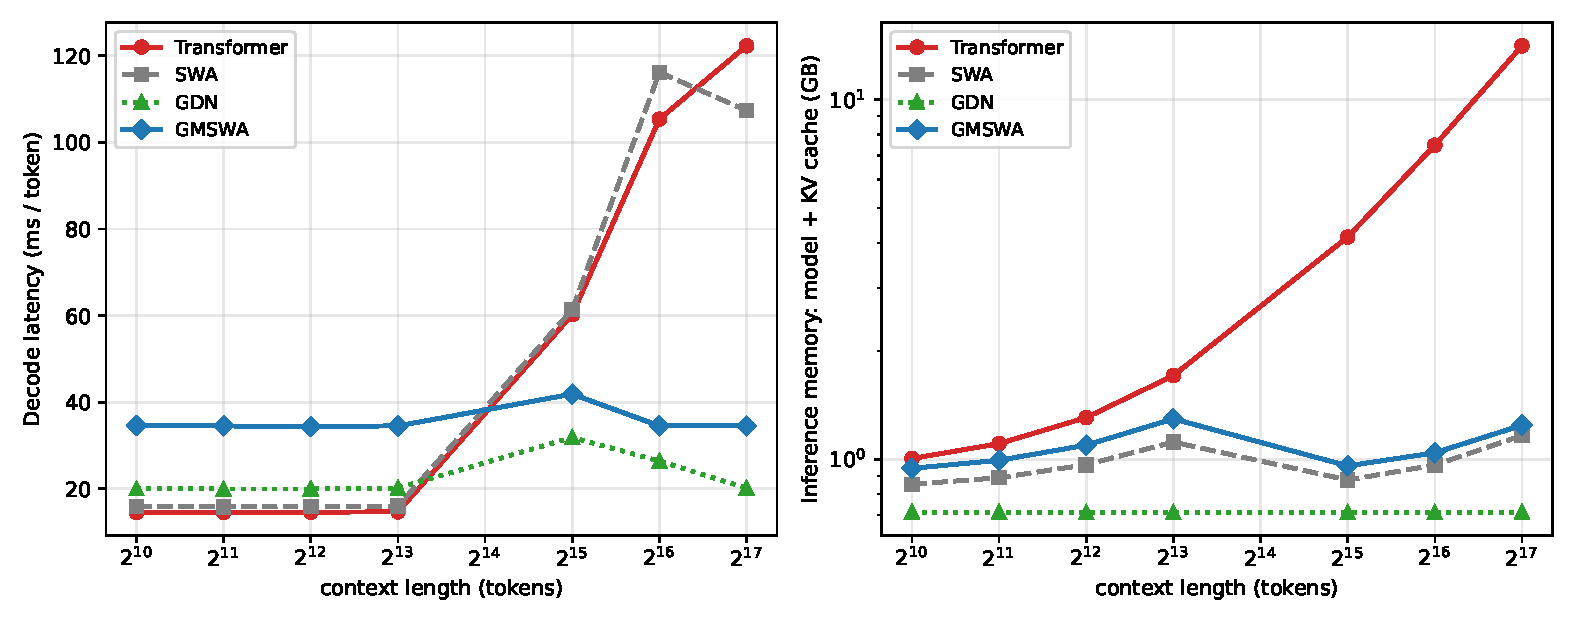
\includegraphics[width=0.92\textwidth]{figures/efficiency.pdf}
\caption{Long-context inference efficiency (340M, bf16, single GPU; decode = median of 3 bursts; $L{=}16$K omitted as a measurement outlier). \textbf{Left:} per-token decode latency. GMSWA and GDN are constant in $L$; the Transformer grows $8.4\times$. The standalone-SWA baseline's growth is a cache-implementation artifact (\S5.3). \textbf{Right:} total inference memory (model${+}$cache, log scale). Transformer grows linearly; GMSWA/SWA/GDN are flat. Analytically, GMSWA's KV cache is a constant $16.3$\,MB vs the Transformer's $12.9$\,GB at 128K (${\sim}790\times$).}
\label{fig:eff}
\end{figure*}

\subsection{Summary}
GMSWA is the only model in our study that is simultaneously (a) competitive on base quality (above recurrent), (b) competitive on real recall (parity with recurrent), and (c) constant in cache and memory (unlike full attention). The one axis on which it does not win is synthetic single-needle recall, examined next.

% ============================================================================
\section{The Synthetic-Recall Limitation: A Negative Result}

\subsection{The gap}
On synthetic single-needle NIAH (Table~\ref{tab:niah}), GMSWA tracks SWA ($0.27$ vs $0.29$ at 2K; $0.16$ vs $0.18$ at 4K) and trails GDN ($0.57$, $0.40$). The gap exists even \emph{within} the training context (2K)---i.e., for needles already beyond the 512 window but inside the trained length---so it is not an extrapolation failure: the window cannot see the needle, and the memory does not perform the sharp single-token retrieval that would compensate, even though it uses the \emph{same} gated-delta kernel GDN uses to succeed.

\subsection{Not gate laziness, not capacity}
Two natural explanations fail. (i) \emph{Gate laziness}: the learned gate is memory-dominant (mean SWA weight $\alpha\approx0.21$), so the memory is heavily used. (ii) \emph{Capacity}: a single needle stores one key$\to$value association---well within a 64-dim head's rank---so the rank wall is not binding. Forcing the mix to memory-only ($\alpha{=}0$) drives NIAH to $0$: the memory alone produces no sharp retrieval, and the (window-limited) recall GMSWA shows is carried by the SWA branch.

\subsection{Five interventions, all negative}
If the memory \emph{could} learn sharp retrieval but is disincentivized, forcing reliance on it should help. We tested five interventions (Table~\ref{tab:ablation}):
\begin{itemize}
\item \textbf{GDN-style output gated-RMSNorm} on the memory readout (v6): \emph{best} perplexity of all models but \emph{collapsed} recall (NIAH${\approx}0$)---normalization smooths away the sharp signal.
\item \textbf{Pathway dropout, aggressive} ($p{=}0.5$, v7): destabilized training (NLL ${\sim}7$--$9$).
\item \textbf{Pathway dropout, gentle} ($p{=}0.15$, v8): degraded everything (NIAH(2048) $0.11$ vs $0.27$; NLL ${\sim}5.4$).
\item \textbf{Memory-first curriculum} (anneal drop $1.0{\to}0$ over 3K steps, v9): a competent LM (NLL ${\sim}4.3$) but NIAH${\approx}0$.
\end{itemize}
Every intervention that shifts reliance toward the memory \emph{hurts}---both recall and perplexity.

\subsection{Explanation: smooth-vs-sharp recall}
The pattern is consistent with a \emph{credit-assignment} effect. Because the window already solves local next-token prediction, the LM objective never \emph{requires} the recurrent memory to perform sharp, exact retrieval; its gradient is dominated by the smooth, long-range, semantic component of the loss. It therefore learns \emph{smooth/semantic} recall---which helps SQuAD and perplexity---but not \emph{sharp synthetic} retrieval. A pure recurrent model (GDN) has no window, so it is \emph{forced} to encode and read recent tokens sharply, and this transfers to single-needle NIAH. Forcing the hybrid's memory to act alone does not create the sharp-retrieval signal absent from the data; it only removes the SWA branch that supplied recall.

We distill a \emph{design caution}: \emph{in window--memory hybrids, the recurrent memory inherits the recall the window leaves on the table---semantic, not synthetic; closing the synthetic gap likely needs a retrieval-explicit objective or a sharper addressing mechanism, not merely forcing memory reliance.}

We scope this carefully. The five interventions establish that \emph{forcing memory reliance does not help} under our LM-training setup at 340M; they do not by themselves prove credit assignment over alternatives (e.g., that the gated-delta kernel with a kernel-4 short-conv cannot address sharply enough). Two cheap experiments would discriminate these and are the natural next step:\todo{(core motivation evidence) train the memory branch ALONE from scratch (architecturally remove SWA, not dropout-mask it) and test NIAH; and a per-branch gradient-norm / per-layer memory-only retrieval probe on the needle token.} we report the credit-assignment reading as our best-supported hypothesis, not a proof.

% ============================================================================
\section{Discussion}
GMSWA delivers a favorable point in the long-context design space: softmax base quality, recurrent-level \emph{real} recall, and a constant cache, with no scale penalty (340M, controlled). Its limitation is precise and explainable. The five-intervention study is, we believe, a useful contribution in its own right: it rules out the obvious fixes and localizes the difficulty to the \emph{kind} of recall the LM objective induces in a hybrid, rather than to capacity or gating.

% ============================================================================
\section{Limitations}
(1) \textbf{Scale, seeds, budget.} All results are at 340M, 10K steps, \emph{single seed}; the close comparisons (zero-shot $0.499$ vs $0.486$; real-recall per-task gaps) are directional, not statistically established---multi-seed runs with confidence intervals are our top revision priority.\todo{run 3 seeds, report $\pm$CI.} Recall is partly scale-emergent, so a 1B study (not completed) could shift the synthetic-recall picture.\todo{1B-scale replication of the negative result.} (2) \textbf{No external-hybrid head-to-head}: we compare Transformer/SWA/GDN but did not retrain a literature hybrid (Griffin/Samba/SWAX-style) under our recipe.\todo{retrain one literature hybrid under the identical recipe.} (3) Real-recall tasks are easier than synthetic single-needle and use low-accuracy regimes. (4) \textbf{Efficiency measurement}: GMSWA decode is ${\sim}2\times$ SWA's (constant in $L$); the harness shows a regime change near 32K and the standalone-SWA decode is an artifact (\S5.3)---the robust claims are the analytical cache reduction and the measured-memory panel. (5) We report token-level NLL because word-perplexity is unreliable under our tokenizer. (6) The credit-assignment account is a hypothesis, consistent with but not proven by the five interventions.

% ============================================================================
\section{Conclusion}
We presented GMSWA, a sliding-window attention fused with a constant-size gated-delta recurrent memory. In a controlled 340M study it preserves softmax base quality (above a recurrent baseline), is comparable to that baseline on real recall (winning two of three tasks), and keeps a constant cache (${\sim}790\times$ smaller KV cache than full attention at 128K). Through five failed interventions we showed that synthetic single-needle recall is hard for such hybrids under standard LM training at this scale, and gave a smooth-vs-sharp recall account of why. GMSWA is thus both a practical constant-cache long-context model and a clean case study of where window--memory hybrids' recall comes from---and where it stops.

% ============================================================================
% ---- TABLES ----
\begin{table}[t]\centering\small
\caption{NIAH single-needle recall vs.\ context length (accuracy; window $W{=}512$). GMSWA tracks SWA and trails GDN; the Transformer collapses past its 2K training length.}
\label{tab:niah}
\begin{tabular}{lccccc}
\toprule
Model & 512 & 1024 & 2048 & 4096 & 8192 \\
\midrule
SWA & 1.00 & 0.65 & 0.29 & 0.18 & 0.08 \\
Transformer & 1.00 & 0.86 & 0.74 & 0.00 & 0.00 \\
GMSWA (ours) & 0.99 & 0.57 & 0.27 & 0.16 & 0.08 \\
GDN (recurrent) & 0.88 & 0.75 & 0.57 & 0.40 & 0.17 \\
\bottomrule
\end{tabular}
\end{table}

\begin{table}[t]\centering\small
\caption{Real recall-intensive tasks (contains-accuracy). GMSWA is comparable to GDN (wins SQuAD/FDA, trails SWDE); both far exceed SWA. Single seed.}
\label{tab:recall}
\begin{tabular}{lccc}
\toprule
Model & SWDE & FDA & SQuAD \\
\midrule
SWA & 0.072 & 0.040 & 0.072 \\
Transformer & \textbf{0.438} & \textbf{0.156} & 0.066 \\
GMSWA (ours) & 0.088 & \textbf{0.094} & \textbf{0.284} \\
GDN & 0.110 & 0.026 & 0.274 \\
\bottomrule
\end{tabular}
\end{table}

\begin{table}[t]\centering\small
\caption{Loss vs.\ token position (token NLL; lower is better). GMSWA is lowest among length-stable models; the Transformer degrades past its 2K training length.}
\label{tab:loss}
\begin{tabular}{lccccc}
\toprule
Model & 0--512 & .5--1K & 1--2K & 2--4K & 4--8K \\
\midrule
SWA & 3.99 & 3.73 & 3.87 & 4.14 & 4.21 \\
Transformer & 3.97 & 3.59 & 3.62 & 5.74 & 7.21 \\
GMSWA (ours) & 3.95 & 3.65 & \textbf{3.78} & \textbf{4.02} & \textbf{4.08} \\
GDN & 4.08 & 3.79 & 3.89 & 4.15 & 4.24 \\
\bottomrule
\end{tabular}
\end{table}

\begin{table}[t]\centering\small
\caption{Standard zero-shot suite (mean accuracy over 10 tasks). All softmax models exceed the recurrent GDN; within-softmax gaps are within single-seed noise.}
\label{tab:zs}
\begin{tabular}{lc}
\toprule
Model & Avg.\ acc.\ (10 tasks) \\
\midrule
Transformer & 0.500 \\
GMSWA (ours) & 0.499 \\
SWA & 0.498 \\
GDN & 0.486 \\
\bottomrule
\end{tabular}
\end{table}

\begin{table}[t]\centering\small
\caption{Per-layer KV cache (bf16, 24 layers; analytical). GMSWA's cache is constant; full attention grows linearly with $L$.}
\label{tab:cache}
\begin{tabular}{lcccc}
\toprule
$L$ & Transformer & SWA & GDN & GMSWA \\
\midrule
8{,}192 & 805\,MB & 50\,MB & 3.4\,MB & 16.3\,MB \\
131{,}072 & \textbf{12{,}885\,MB} & 50\,MB & 3.4\,MB & \textbf{16.3\,MB} \\
\bottomrule
\end{tabular}
\end{table}

\begin{table}[t]\centering\small
\caption{Recall ablation: five interventions on GMSWA (all 340M, identical recipe). Every change that shifts reliance toward the memory hurts both recall and perplexity.}
\label{tab:ablation}
\begin{tabular}{lccc}
\toprule
Variant & NIAH(2K) & SQuAD & NLL \\
\midrule
GMSWA (final) & \textbf{0.27} & \textbf{0.284} & ${\sim}3.9$ \\
\;+ output gated-RMSNorm & 0.01 & 0.022 & ${\sim}3.7$ \\
\;+ SWA-dropout $p{=}0.5$ & 0.00 & 0.024 & ${\sim}7$--$9$ \\
\;+ SWA-dropout $p{=}0.15$ & 0.11 & 0.160 & ${\sim}5.4$ \\
\;+ memory-first curriculum & 0.00 & 0.140 & ${\sim}4.3$ \\
\bottomrule
\end{tabular}
\end{table}

% NOTE: aaai2026.sty already issues \bibliographystyle{aaai2026}; do not repeat it.
\bibliography{references}

\end{document}
